\section{System Architecture} \label{sec:sysarc}


The LSST control system is based on a reactive data-driven actor-based architecture that uses a multi cast Data Distribution Service (DDS) messaging protocol middleware. A high level view of this architecture is given in \figref{fig:arc}, where each box corresponds to a component of the system (not all components are displayed here). 

The LSST System Architecture is comprised mainly of;
%
\begin{itemize}
\item The Service Abstraction Layer (SAL\footnote{\url{https://docushare.lsstcorp.org/docushare/dsweb/Get/Document-21527/}}) communication middleware. Based on the DDS protocol, it provides interfaces for all the project adopted programming languages (LabView, C++, Java and Python).
\item Engineering and Facility Database (EFD).
\item SAL-aware reactive components, a.k.a Commandable SAL Components (CSCs). 
\item LSST Operators Visualization Environment (LOVE).
% \item Python SalObj\footnote{\url{https://github.com/lsst-ts/ts_salobj}} library.
%\item LabView component template. 
% \item Script Queue  \footnote{\url{https://github.com/lsst-ts/ts_scriptqueue}}
\end{itemize}

\begin{figure}
\begin{center}
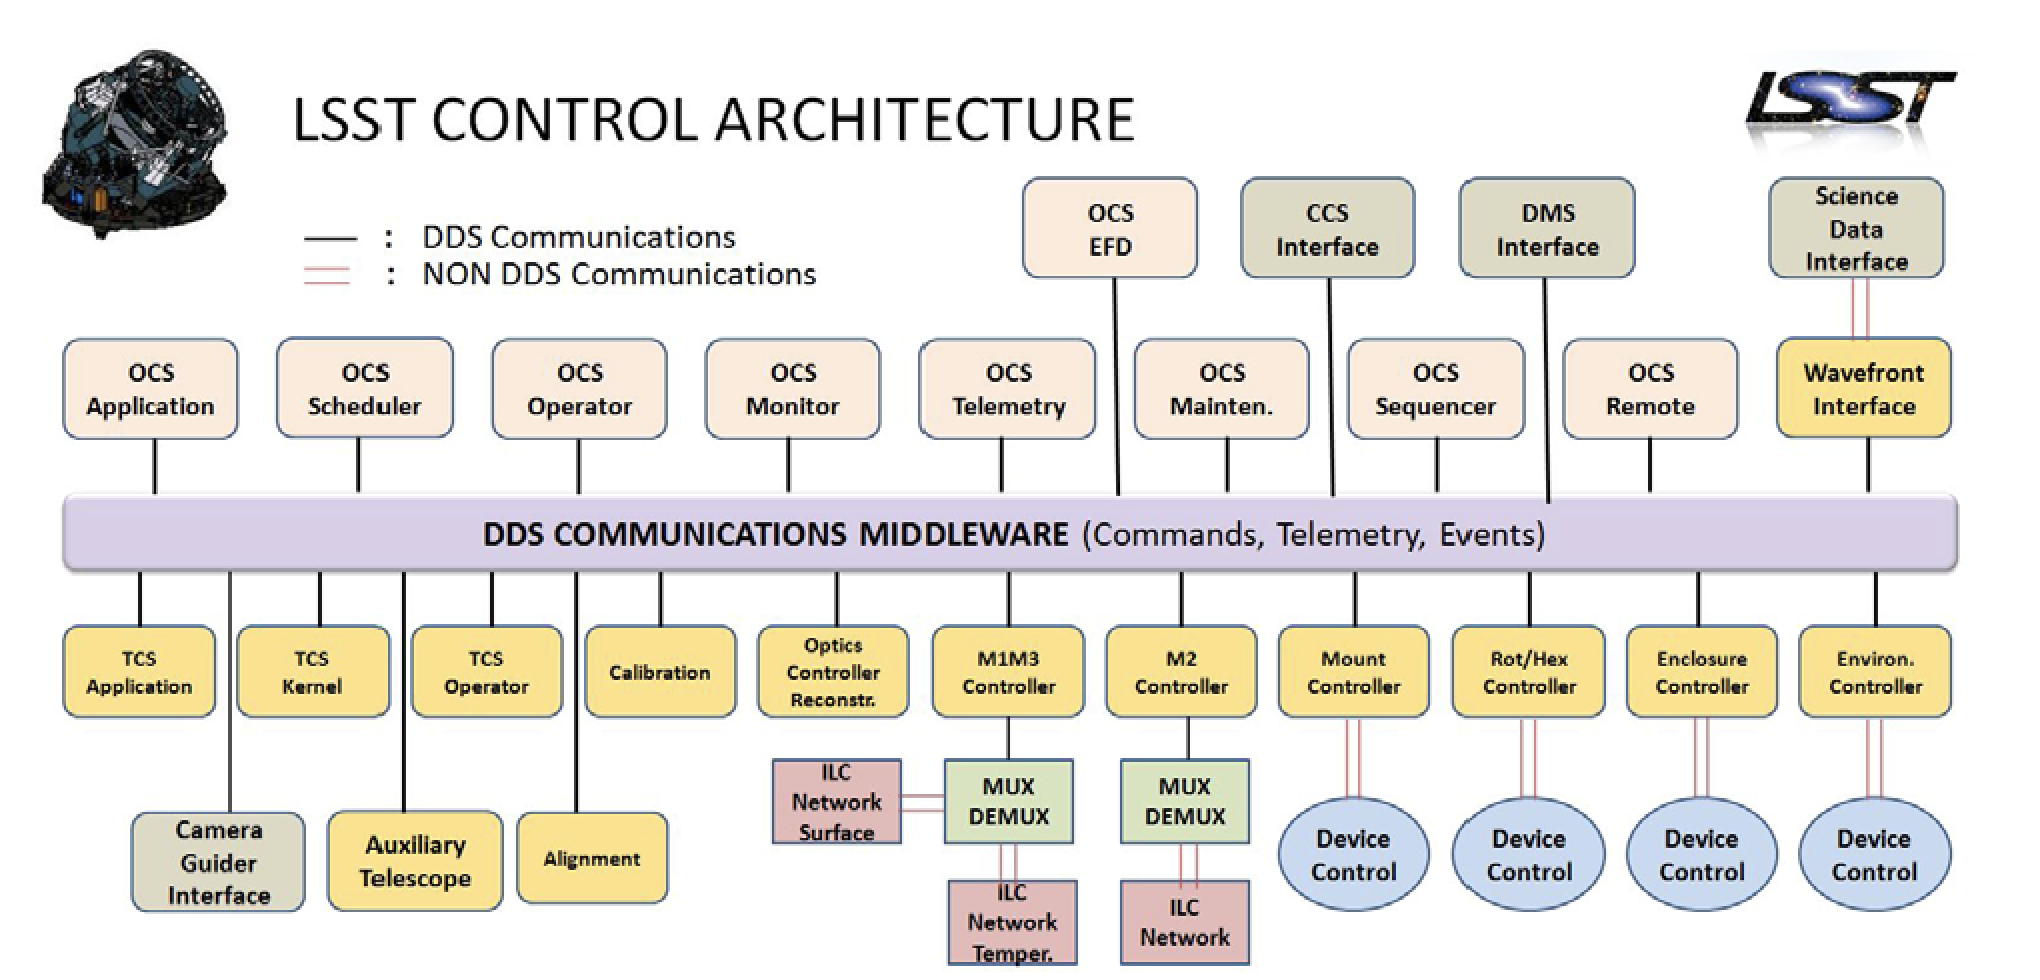
\includegraphics[width=0.8\textwidth]{arc}
\caption{High Level Architecture Diagram\label{fig:arc}}
\end{center}
\end{figure}

The SAL middleware is the backbone of the LSST system architecture. It implements three distinct types of messages; Commands, Events and Telemetry, with distinct purposes. Commands are sent to a specific component, which must acknowledge its receipt and perform some action. In general, the receiving component will be the only entity listening for the commands it accepts. Events and Telemetry are messages broadcasted by components to the middleware and are available to any entity on the system to receive. The distinction between Events and Telemetry is that the former receives a higher priority by the message passing systems. 

The EFD is responsible for capturing all SAL messages broadcasted to the middleware (including Commands, Events and Telemetry) and storing that information into a database. 

CSCs are the main actors of the LSST system architecture. They are responsible for managing the incoming traffic of data and take appropriate actions, controlling hardware (e.g. M1M3, M2, Mount Controller, etc in Fig.~\ref{fig:arc}), software (e.g. Optics Controller Reconstructor, DMCS Interface, etc in Fig.~\ref{fig:arc}) or even other CSCs (e.g. Script Queue, TCS, ATCS, OCS, etc in Fig.~\ref{fig:arc} ).

LOVE is responsible for capturing SAL messages and displaying them in a useful way for general users, providing some basic interface to query and analyze data from the EFD and an interface to issue some pre-defined commands to a set of components.

One of the fundamental parts of SAL is to provide a low-level API for publishing and subscribing to the middleware. These APIs are generated for each component independently, based on pre-defined interfaces. On top of those low level APIs, developers have access two higher level set of frameworks; Python SalObj\footnote{\url{https://github.com/lsst-ts/ts_salobj}} library and the LabView component template. No higher level framework is supported for implementation in Java or C++. 

% a Python library (e.g. SalObj) or the LabView component template. There is no higher level support for implementation in Java or C++. 

% Each component of the system is and independent actor that reacts to data published to the middleware. 

%\begin{itemize}
%\item Infrastructure and Middleware :
%\item The Scheduler \footnote{\url{https://github.com/lsst-ts/ts_scheduler}}
%\item Potentially an Auxiliary and Main Telescope Control System (ATCS and TCS)\footnote {The precise nature and need for these is unclear now so they have lower priority.}
%\item Controllable SAL Components (CSCs) - every device and some pseudo devices, including the scheduler, are CSCs. Some are coordinating other CSCs, the full hierarchy is shown for AuxTel in \figref{fig:atcscs} and the Main Telescope in \figref{fig:mtcscs}
%\end{itemize}

Overall, the system architecture can be divided into three main namespaces; Observatory, Main Telescope (MT) and Auxiliary Telescope (AT). The Observatory is the highest level and encapsulates both the Main Telescope, Auxiliary Telescope and global components such as the weather station, DIMM, etc. The complete set of components that belong to each of these namespaces can be seen in Figs.~\ref{fig:ocs}, ~\ref{fig:atcscs} and \ref{fig:mtcscs}.

\begin{figure}
\begin{center}
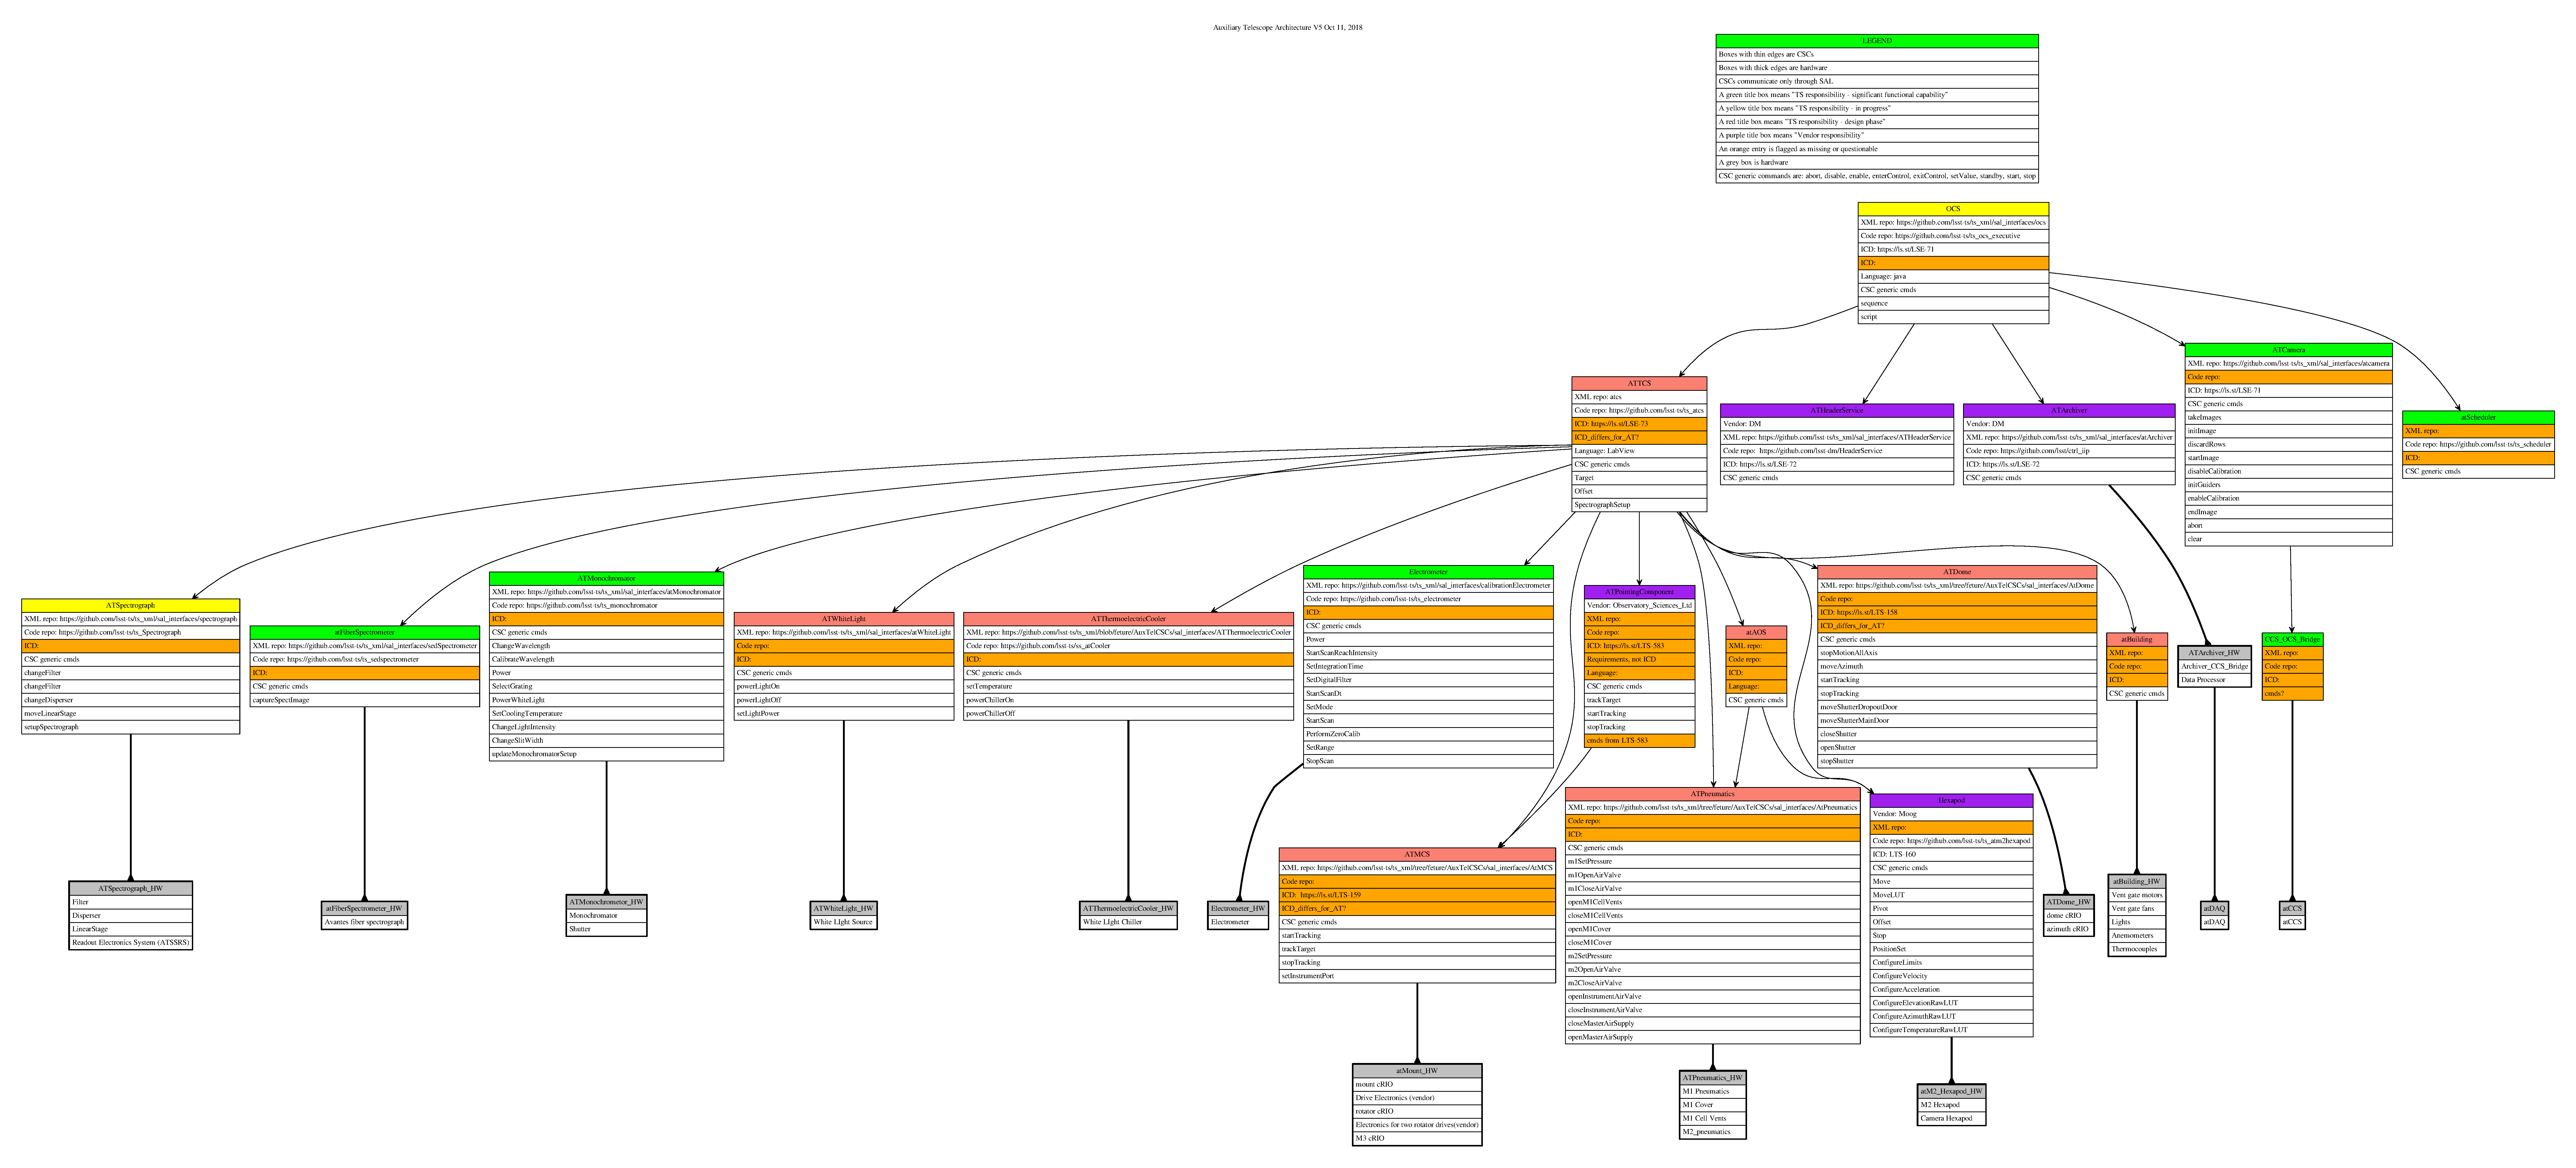
\includegraphics[width=0.9\textwidth]{AT}
\caption{Complete set of AT CSCs\label{fig:atcscs}}
\end{center}
\end{figure}

\begin{figure}
\begin{center}
\includegraphics[width=0.9\textwidth]{LSST}
\caption{Complete set of MT CSCs\label{fig:mtcscs}}
\end{center}
\end{figure}

\subsection{SalObj - Python and scripting }\label{sect:salobj}
SalObj is a Python library provides a pythonic and object-oriented interface to create CSCs and Scripts that can be executed by the script queue component (see Sect.~\ref{sect:scriptq}). The library defines two sets of base classes that are mirror to each other, Remote and Controller. A Remote will send commands to and receive telemetry and events from a specific component whereas a Controller will receive commands and publish telemetry and events. In this framework, a CSC is a specialized Controller that is configure to perform some basic actions by default. A high level diagram is provided in \figref{fig:salobj}.

Internally, SalObj uses the python library asyncio\footnote{\url{https://docs.python.org/3/library/asyncio.html}} to handle the inherently asynchronous nature of the SAL messaging system. 

\begin{figure}
\begin{center}
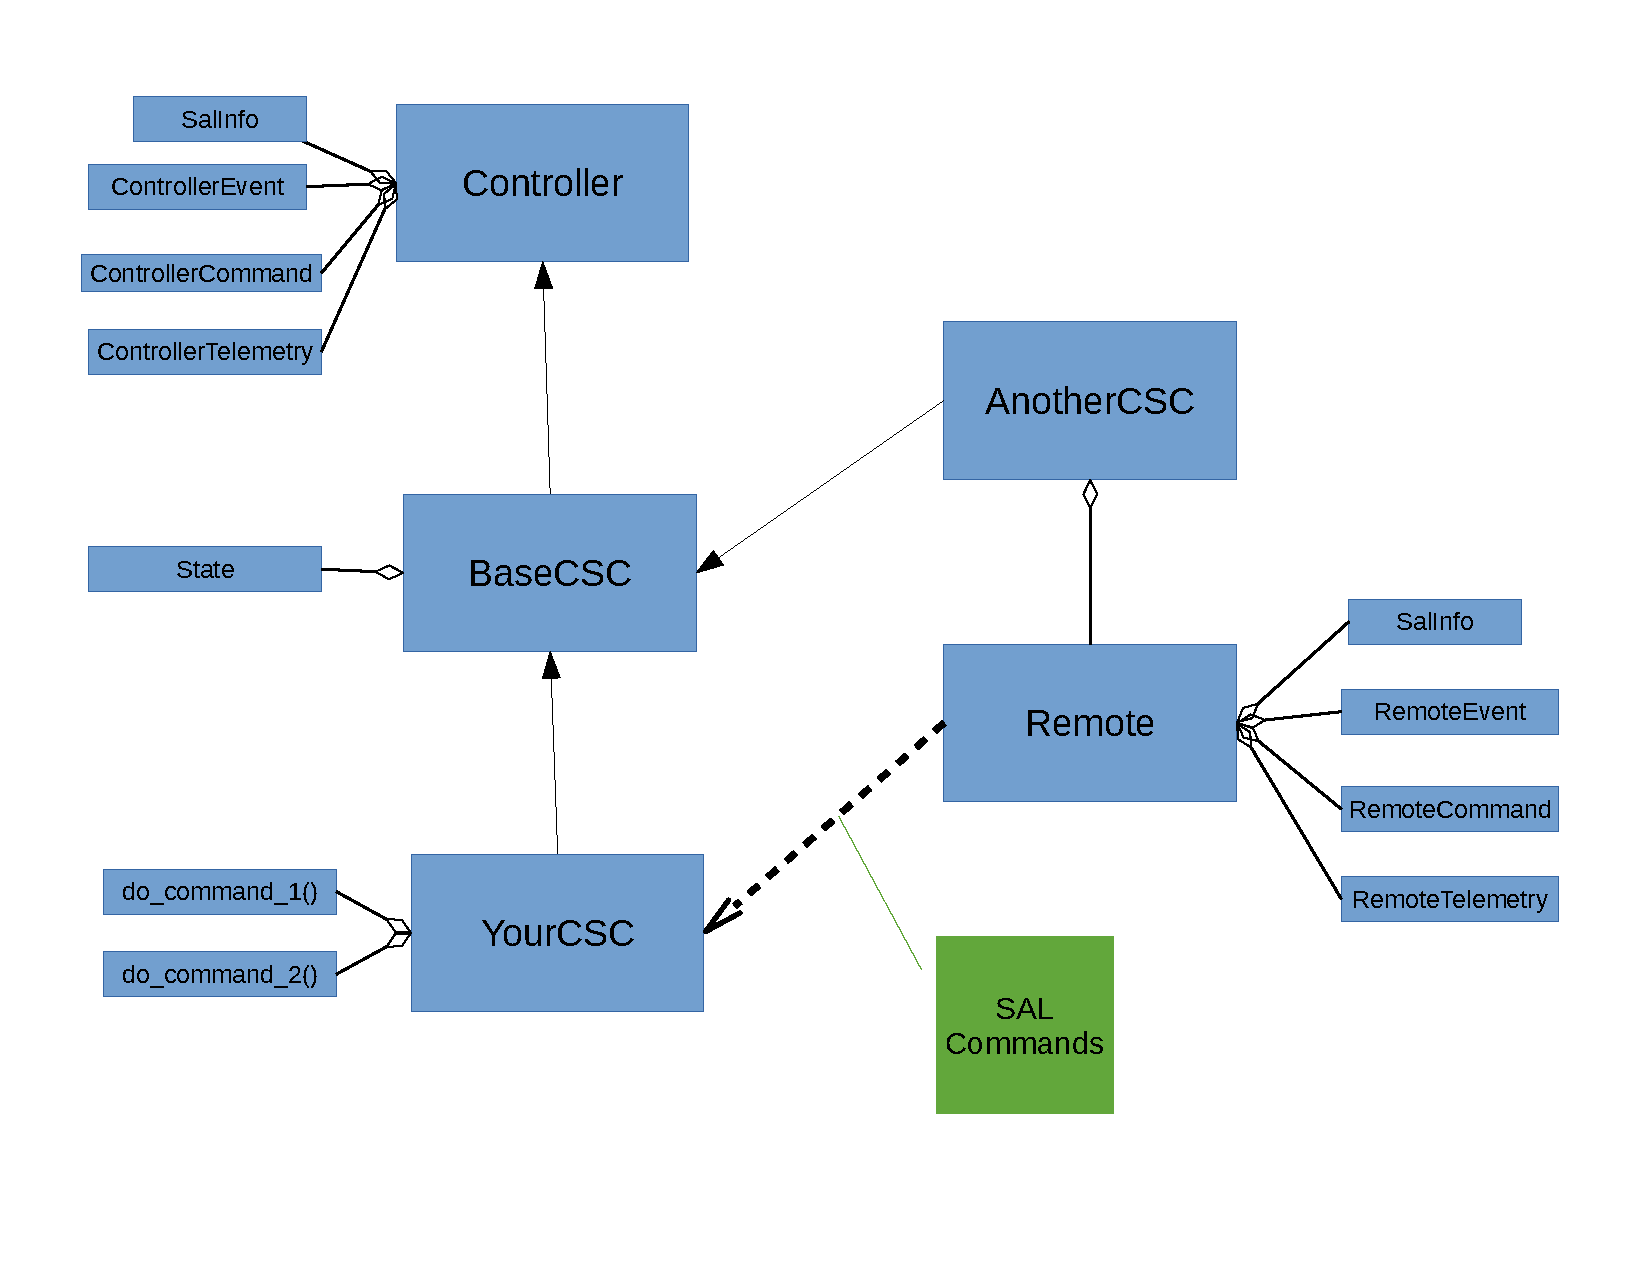
\includegraphics[width=0.9\textwidth]{SalobjClassDiag2}
\caption{SalObj python scheme for  CSCs\label{fig:salobj}}
\end{center}
\end{figure}

\subsection{ScriptQueue} \label{sect:scriptq}
There are a number of different ways users can interact with components in the LSST system. For instance, one could easily use the SAL generated API in any of the supported languages to send commands directly to a single or multiple components. It is also possible to use SalObj Remotes to write Python scripts that would command different components to accomplish a specified task. Not to mention that LOVE itself provides a customizable interface for users to interact with components. 

Nevertheless, during commissioning and operations the LSST system will require a high degree of coordination between different crews (different daytime and nighttime shifts, for instance), not to mention the increasing number of available components and level of complexity as the system ramps up. In order to manager those issues, the LSST control system contains a specialized script queueing component, a.k.a. the ScriptQueue\footnote{\url{https://github.com/lsst-ts/ts_scriptqueue}}.

The ScriptQueue defines an interface for developing scripts in general, and provides a basic class that can be used to develop Python scripts. As Python programs, these scripts have access to all Python functionality, both from the native Python 3 language and through imported modules (including asyncio to manage concurrent activities or libraries from the DM stack). In particular, a Script has access to all the system components using SalObj Remotes (\secref{sect:salobj}) . Although Python is the only language officially supported, scripts can be written in any SAL-supported language. As long as they follow the interface defined by the ScriptQueue component, it should be possible to execute them. 

\subsection{Observatory Control System } \label{sect:ocs}
In such an environment it is not immediately clear that a traditional hierarchical design is necessary or desirable. A completely flat architecture initially seems completely workable and certainly sufficient during in AIT and early commissioning. For example, consider a Script which commands and sequences the telescope subsystems to move to the next field to be observed, take an exposure, and read out that exposure. The Script can directly control each of those subsystems and maintain control of the sequencing using asyncio. Furthermore, the complexity of the Script can be managed through normal modular programming techniques, in which subsystem functionality is implemented through Python objects imported in modules.

Though we could have a flat system based on ScriptQueue (\secref{sect:scriptq})
there are two compelling reason to retain at least a top level OCS which has
overall responsibility for all subsystems. The first reason is rooted in the limited lifetime of each
Script, which has an execution thread that begins and ends over a duration short compared to
the up time of the telescope system. When a Script is instantiated, it has no immediate
knowledge of the state of the telescope system as a whole, or the state of individual
subsystems. It needs such knowledge, because many actions, e.g. moving the telescope,
require the telescope subsystems to be in particular states. The Script can of course assemble
the required knowledge, by using SAL to obtain the state information of all relevant subsystems,
but doing so imposes unnecessary startup overheads for Scripts. It is far more efficient, not to
say reliable, for a single subsystem to be continuously responsible for maintaining knowledge of
the overall state of the observatory (observatory states are discussed in more detail below)

The second, related, reason is that the operator needs:
\begin{enumerate}
\item to maintain continuous knowledge of
the state of the observatory independent of Script execution, and
\item  to be able to command the
observatory to change its overall state.
\end{enumerate}
An excellent example of the latter requirement is from
the LOVE requirements document, \citeds{LTS-807}: “The LOVE shall provide a single control
command labeled “Emergency Close” of the telescopes”. Certainly one could imagine creating
a Script to execute “Emergency Close”, but to use it would require that any currently running
Script be aborted, and the “.

It should be noted this could also be achieved by an "Emergency Close" script inserted on top of the ScriptQueue and an abort on the current running script (if there is one) - the ScriptQueue supports this.  So the OCS remains a low priority to be developed during commissioning as we understand the needs better.
